\chapter{Design}
Now we will design how to implement what we have defined in the analysis chapter.
Our application is a single-page web application.

\section{Architecture}
\begin{figure}[h]
  \centering
  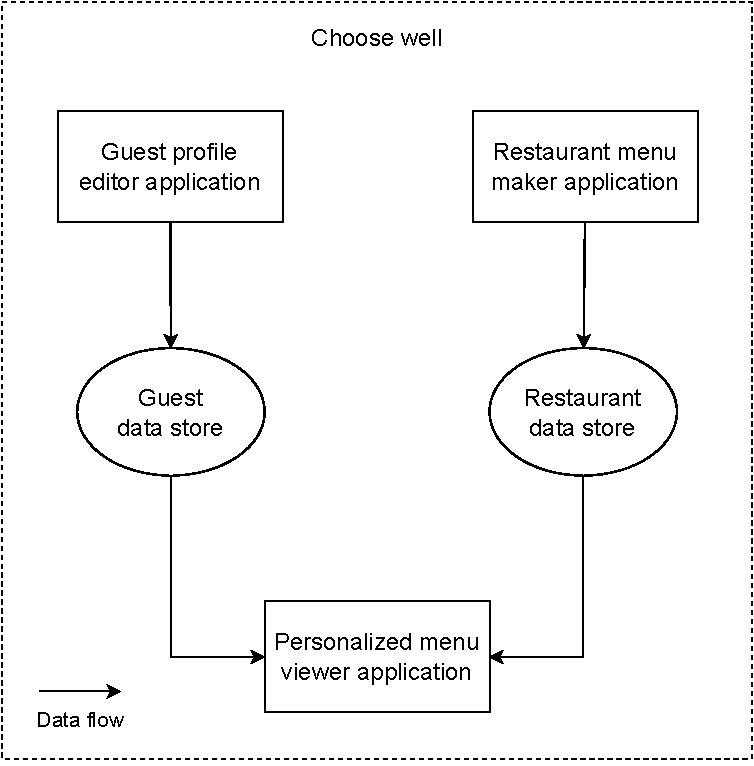
\includegraphics[width=0.62\linewidth]{master-thesis/img/architecture_data_flow.pdf}
  \caption{Application's data flow diagram}
\end{figure}

\section{Technological stack}
There are various options out there for what technologies we can use to implement our application.
This section contains an overview of available tools and which ones we chose and why.

\subsection{Front-end}
Nowadays, there are many frameworks for building web applications.
We need to be able to create an interactive user interface.
We need to have state for logged in user.
We need to fetch data from the internet.
We need to integrate with Solid.
The most popular are listed below with their pros and cons.

\subsubsection*{Angular}
Angular is a platform and framework for building single-page client applications using HTML and TypeScript. 
It implements its core and optional functionality as a set of TypeScript libraries. 
The basic building blocks of the Angular framework are Angular components that are organized into \emph{NgModules}. 
NgModules collect related code into functional sets; an Angular application is defined by a set of NgModules.

\subsubsection*{React.js}
React is a JavaScript library for rendering user interfaces.
Applications written in React are built from modular and reusable pieces called components.
React components receive data and return what should appear on the screen. 
They can be passed new data in response to an interaction, like when the user types into an input. 
React will then update the screen to match the new data.
A notable feature is the use of a virtual Document Object Model, or Virtual DOM. 
React creates an in-memory data-structure cache, computes the resulting differences on a re-render, and then updates the browser's displayed DOM efficiently. 
This selective rendering provides a major performance boost.

\subsubsection*{Vue.js}

As for programming languages, we consider two options. 

\begin{description}
  \item[JavaScript] 
  \item[TypeScript] 
\end{description}

% react router

\subsection{nasadenie}
%  Vite, npm
% create react app, webpack, yarn

\subsection{Responsive design}
We need our application to be responsive to various device screens.
\begin{description}
  \item[Bootstrap] 
  \item[Material UI] 
\end{description}

\subsection{Persistence}
We need to store and later read data.
% Solid pods

\subsection{Testing}
We need to test our application in order to prevent bugs during implementation.
% https://legacy.reactjs.org/docs/testing-environments.html

\subsection{Documentation}
We need to capture how our application works for users and future developers.
% (GitHub markdown)

\section{Wireframes}
\begin{figure}[h]
  \centering
  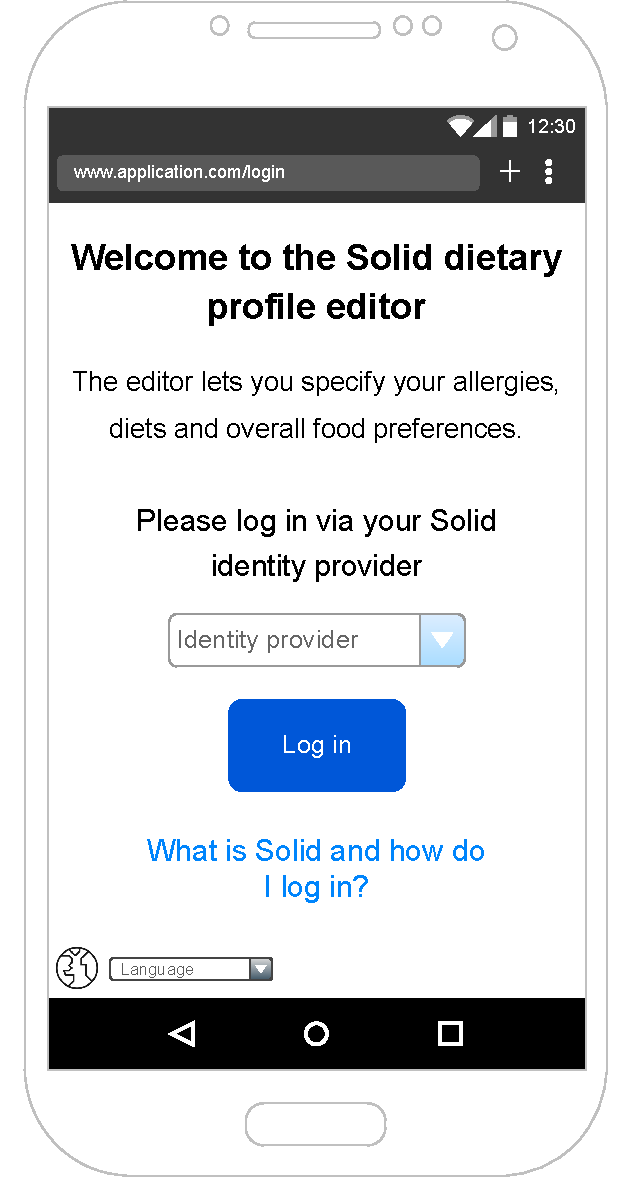
\includegraphics[width=0.62\linewidth]{master-thesis/img/wireframes/guest_profile_editor/login.pdf}
  \caption{Guest profile editor login screen}
\end{figure}

\begin{figure}[h]
  \centering
  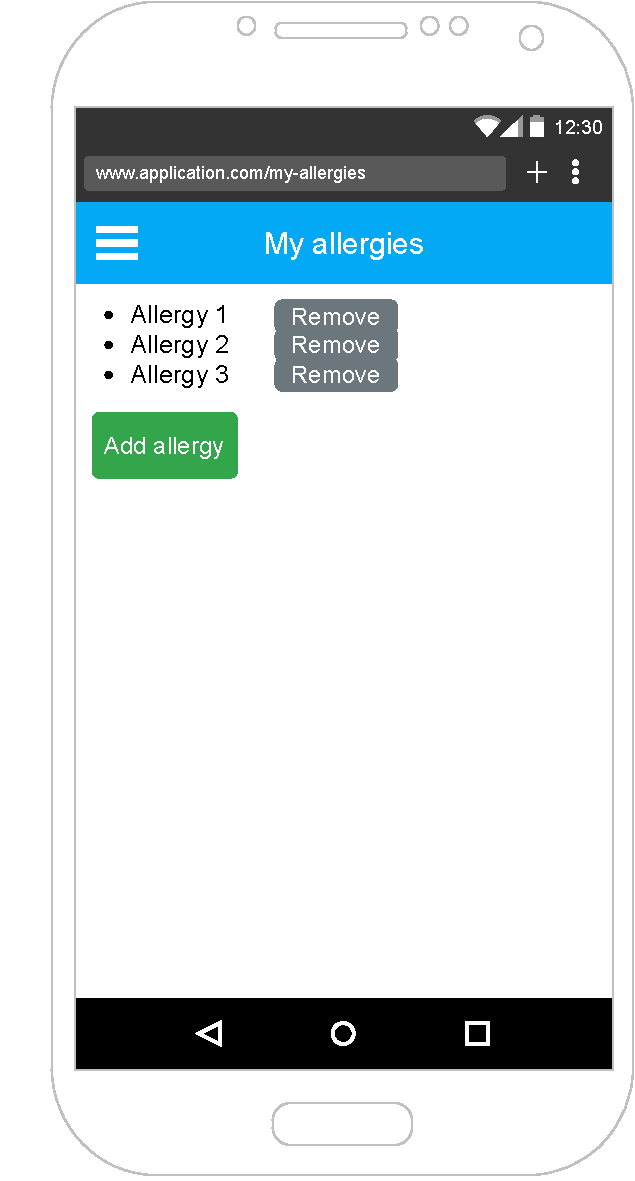
\includegraphics[width=0.62\linewidth]{master-thesis/img/wireframes/guest_profile_editor/my_allergies.pdf}
  \caption{Guest profile editor allergies screen}
\end{figure}

\begin{figure}[h]
  \centering
  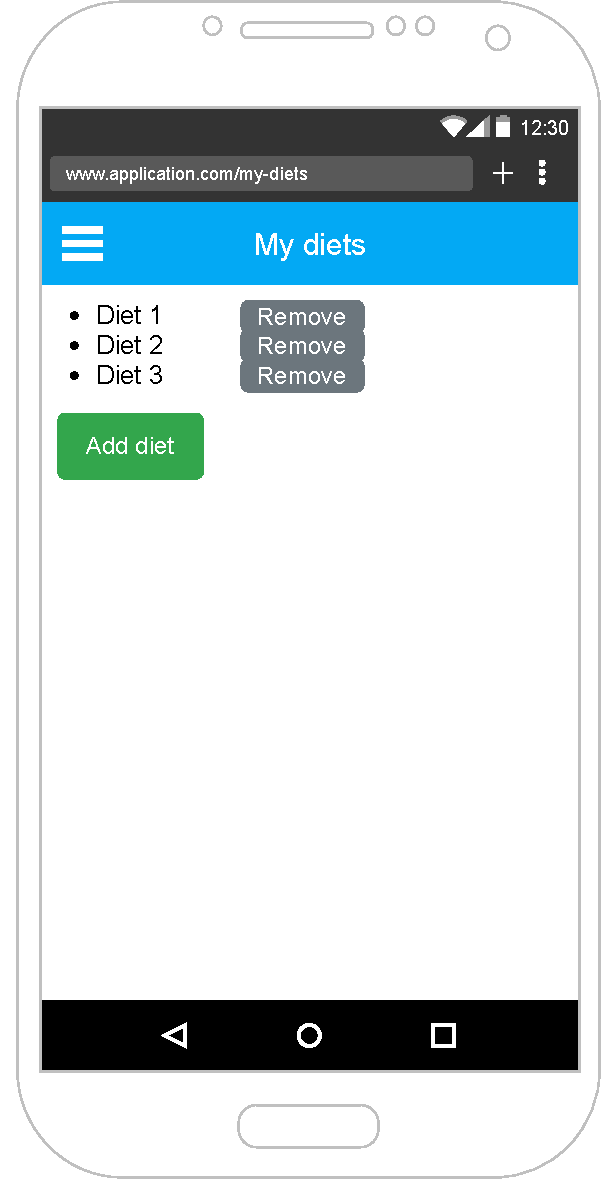
\includegraphics[width=0.62\linewidth]{master-thesis/img/wireframes/guest_profile_editor/my_diets.pdf}
  \caption{Guest profile editor diets screen}
\end{figure}

\begin{figure}[h]
  \centering
  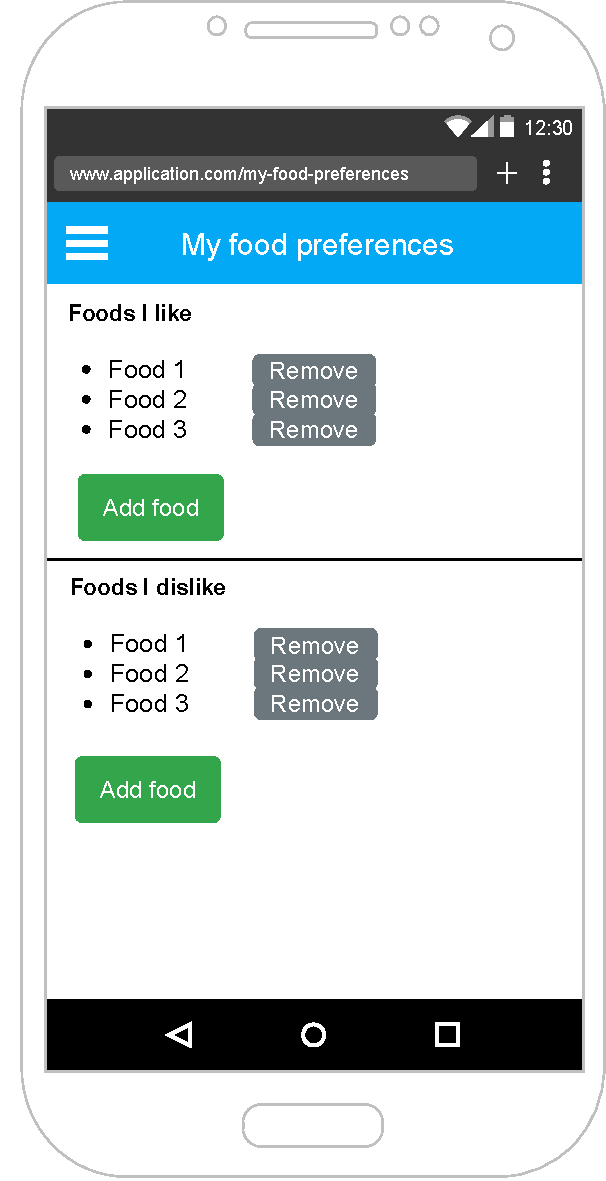
\includegraphics[width=0.62\linewidth]{master-thesis/img/wireframes/guest_profile_editor/my_food_preferences.pdf}
  \caption{Guest profile editor food preferences screen}
\end{figure}

\begin{figure}[h]
  \centering
  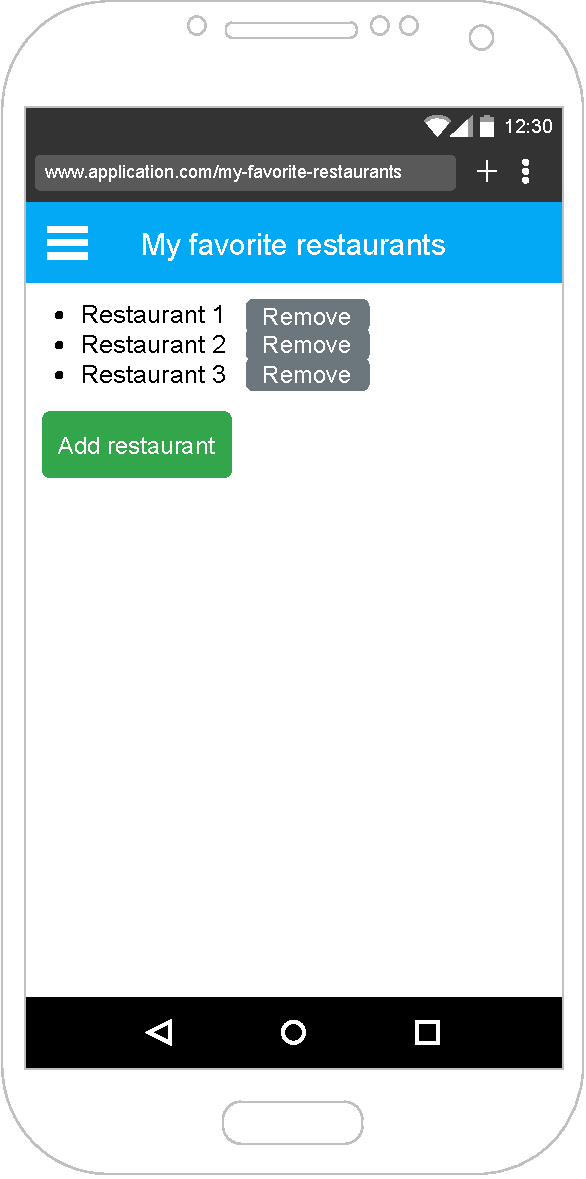
\includegraphics[width=0.62\linewidth]{master-thesis/img/wireframes/guest_profile_editor/my_favorite_restaurants.pdf}
  \caption{Guest profile editor favorite restaurants screen}
\end{figure}

\begin{figure}[h]
  \centering
  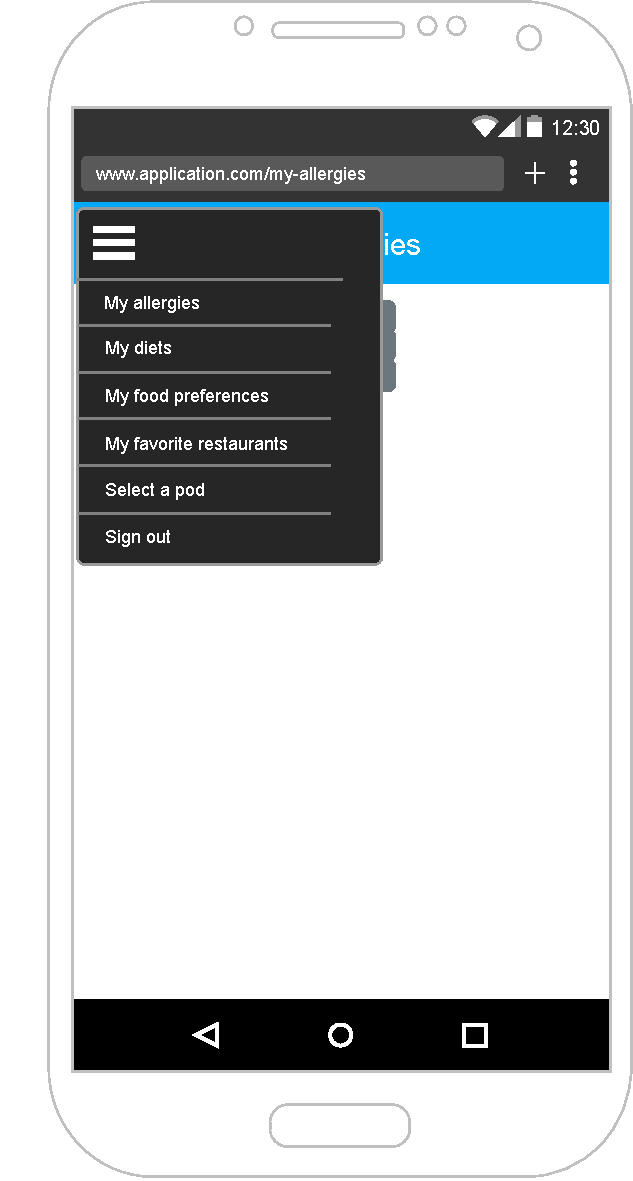
\includegraphics[width=0.62\linewidth]{master-thesis/img/wireframes/guest_profile_editor/menu_expanded.pdf}
  \caption{Guest profile editor screen with expanded menu}
\end{figure}

\listoftodos